\documentclass[12pt]{beamer}
\usepackage[T2A]{fontenc}
\usepackage[utf8]{inputenc}
\usepackage[english,russian]{babel}
\usepackage{amssymb,amsfonts,amsmath,mathtext}
\usepackage{cite,enumerate,float,indentfirst}
\usepackage{wrapfig} % Text wrapping around figures
\usepackage{pscyr} % Нормальные шрифты

\graphicspath{{images/}}

\usetheme{Singapore}
%\usecolortheme{whale}

\setbeamertemplate{navigation symbols}{} %remove navigation symbols at all
\setbeamercolor{footline}{fg=black}
\setbeamerfont{footline}{size=\fontsize{8}{10}\selectfont}
\setbeamersize{text margin left=0.6cm, text margin right=0.4cm}
\setbeamertemplate{footline}{
  \leavevmode%
  \hbox{%
%    \begin{beamercolorbox}[wd=.5\paperwidth,ht=2.5ex,dp=1ex,left]{}%
%      Я. А. Воронцов, ВГУ
%    \end{beamercolorbox}%
    \begin{beamercolorbox}[wd=\paperwidth,ht=2.5ex,dp=1ex,right]{}%
      \insertframenumber{} / \inserttotalframenumber \hspace*{2ex}
    \end{beamercolorbox}
  }%
  \vskip0pt%
}

\newcommand{\itemi}{\item[\checkmark]}

\title{\Large{Математическое моделирование задач выбора с расплывчатой неопределенностью на основе методов представления и алгебры нечетких параметров}}
\author{\normalsize{%
Я. А. Воронцов\\%
\emph{Научный руководитель:}~М.Г.Матвеев,~д.т.н.,~профессор.}\\%
\small{
\vspace{2pt}
Специальность 05.13.18~--- математическое моделирование,\\ численные методы и комплексы программ \\
\vspace{2pt}
ФГБОУ ВПО <<Воронежский государственный университет>>%
\vspace{10pt}%
}
\small{Воронеж, 2015}
}

\begin{document}

\maketitle

%%%%%%%%%%%%%%%%%%%%%%%%%%%%%%

\begin{frame}
  \frametitle{Классификация нечётких моделей}
  \begin{columns}[onlytextwidth]
    \begin{column}{0.6\textwidth}
      \begin{figure}[h]
        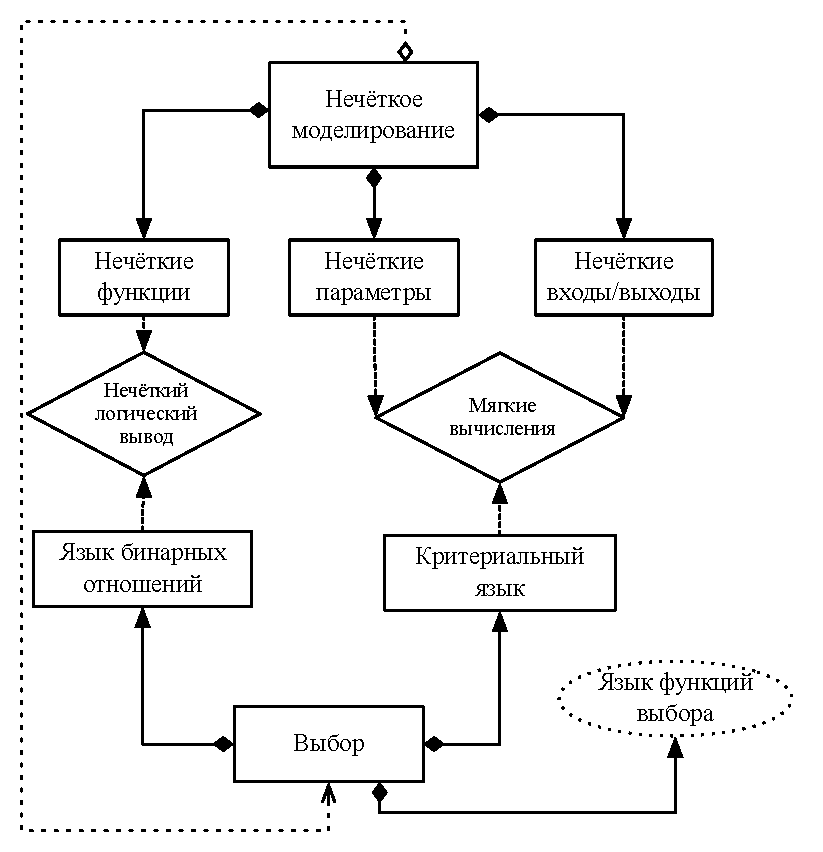
\includegraphics[width=\textwidth]{choice-classification}
      \end{figure}
    \end{column}
    \begin{column}{0.4\textwidth}
      \begin{itemize}
        \item Исследуются модели, использующие чёткие отношения и нечёткие параметры (модели второго типа)
        \item Существующие подходы к нечётким вычислениям далеко не всегда применимы в моделях второго типа
      \end{itemize}
    \end{column}
  \end{columns}
\end{frame}

%%%%%%%%%%%%%%%%%%%%%%%%%%%%%%

\begin{frame}
  \frametitle{Особенности существующих способов мягких вычислений}
  \begin{itemize}
    \item требуются значительные вычислительные ресурсы;
    \item неоправданно расширяется носитель функции принадлежности;
    \item происходит выход за класс используемых в арифметике чисел из-за искажения формы функции принадлежности;
    \item ограничивается область определения функции принадлежности;
    \item нарушаются классические отношения равенства и частичного порядка.
  \end{itemize}
\end{frame}

%%%%%%%%%%%%%%%%%%%%%%%%%%%%%%

\begin{frame}
  \frametitle{Цель и задачи исследования}
  \textbf{Цель:} построение и исследование моделей учёта нечёткой неопределённости, обеспечивающих требуемые свойства решения различных прикладных задач, а также разработка методов эффективного численного решения на основе вводимых моделей \\
  \textbf{Задачи:}
  \begin{itemize}
    \item анализ существующих методик нечётких вычислений с~точки зрения сохранения свойств решения задач;
    \item разработка модели представления нечётких чисел, позволяющей максимально сохранять исходную экспертную информацию и обеспечить требуемые качественные свойства решений (устойчивость, сохранение чётких математических соотношений и т.\,п.);
  \end{itemize}  
\end{frame}

%%%%%%%%%%%%%%%%%%%%%%%%%%%%%%

\begin{frame}
  \frametitle{Цель и задачи исследования}
  \textbf{Задачи:}
  \begin{itemize}
    \item разработка методики эффективной численной реализации решения задач с нечёткими параметрами, основанной на подходящих алгебраических структурах и её тестирование на примере задачи сетевого планирования с нечёткими параметрами;
    \item разработка и верификация программного обеспечения, реализущего предложенную модель представления нечётких параметров и методики численного решения задач с нечёткими параметрами.
  \end{itemize}  
\end{frame}

%%%%%%%%%%%%%%%%%%%%%%%%%%%%%%

\begin{frame}
  \frametitle{Представление нечёткой информации}
  \begin{itemize}
    \item нечёткие множества (подмножества предопределённого универсального множества X)
      \begin{equation}
      	\tilde{A}=\left\{ \left( x, \mu_{\tilde A}\left( x \right) \right)\left| x\in X \right. \right\};\ E \left( \mu_{\tilde A} \left( x \right) \right) = \left[0; 1 \right]
      \end{equation}      
    \item нечёткие числа (подмножества множества $\mathbb{R}$)
      \begin{itemize}
        \item кусочная непрерывность $\mu_{\tilde A}\left( x \right)$;
        \item выпуклость $\mu_{\tilde A}\left( x \right)$
      	\begin{gather}
      	  \forall x_1, x_2 \in \mathbb{R}; \forall \gamma \in \left[ 0;1 \right] \notag \\
      	  \mu_{\tilde A}\left( \gamma x_1+\left( 1-\gamma  \right)x_2 \right)\geqslant \min \left\{ \mu_{\tilde A}\left( x_1 \right),\mu_{\tilde A}\left( x_2 \right) \right\}
      	\end{gather}
      	\item нормальность $\mu_{\tilde A}\left( x \right)$
        	\begin{equation}
        		\underset{x\in \mathbb{R}}{\mathop {\sup}}{}\, \left( \mu_{\tilde A} \left( x \right) \right)=1
        	\end{equation}
      \end{itemize}
  \end{itemize}
\end{frame}

%%%%%%%%%%%%%%%%%%%%%%%%%%%%%%

\begin{frame}
  \frametitle{Основные понятия}
  \begin{itemize}
    \item Треугольное нечёткое число $\tilde A = \left\langle m,a,b \right\rangle $
      \begin{equation}
        \mu_{\tilde A}\left( x \right)=
        \left\{ \begin{aligned}
			& \frac{x-m+a}{a};\ x\in \left[ m-a;m \right] \\ 
			& \frac{m+b-x}{b};\ x\in \left( m;m+b \right] \\ 
			& 0;\ \text{в остальных случаях} 
	 	\end{aligned} \right.
      \end{equation}
    \item Число как совокупность $\alpha$-интервалов $X_\alpha = \left[x^L(\alpha); x^R(\alpha) \right]$
      \begin{equation}
        \left[ 
          \begin{aligned}
            & x^L(\alpha )=m-a+a\alpha  \\ 
            & x^R(\alpha )=m+b-b\alpha
          \end{aligned}
        \right.
      \end{equation}
    \item Число $LL$ $\left( RR \right)$-типа~--- правый (левый) коэффициент нечёткости числа равен нулю
  \end{itemize}
\end{frame}

%%%%%%%%%%%%%%%%%%%%%%%%%%%%%%

\begin{frame}
  \frametitle{Преобразование L}
  \begin{itemize}
    \item Переход к интервальной неопределенности
      \begin{equation}
        \label{eq:task-transform}
      	\tilde{Y} = f\left( \tilde X, \tilde A \right)\to \bigcup\limits_{\alpha =0}^{1}{y_\alpha}=f\left( X_\alpha, A_\alpha \right)
      \end{equation}
    \item Переход к чётким значениям на каждом $\alpha$-уровне 
      \begin{equation}
        \label{eq:L-transform-base}
        \bar{x}\left( \alpha  \right)=L\left( X_\alpha \right)=\lambda x^L \left( \alpha  \right)+\left( 1-\lambda  \right) x^R \left( \alpha  \right);\, \lambda \in \left[0; 1 \right]
      \end{equation}
    \item Модифицированное решение
      \begin{equation}
        \tilde Y^{*}= \bigcup\limits_{\alpha =0}^{1} f\left(L\left( X_\alpha \right), L\left( A_\alpha \right) \right)=\left\{ y_\alpha \left| \mu_{\tilde Y^*}(y)=\alpha \right. \right\}
      \end{equation}
    \item Модифицированное нечёткое число (LL/RR-типа)
      \begin{equation}
        \label{eq:modified-number}
        \mu_{\tilde A^{*}}\left( x \right)={\left( \bar{x}\left( \alpha  \right) \right)}^{-1}
      \end{equation}
  \end{itemize}
\end{frame}

%%%%%%%%%%%%%%%%%%%%%%%%%%%%%%

\begin{frame}
  \frametitle{Преобразование L}
  \begin{figure}
    \center
    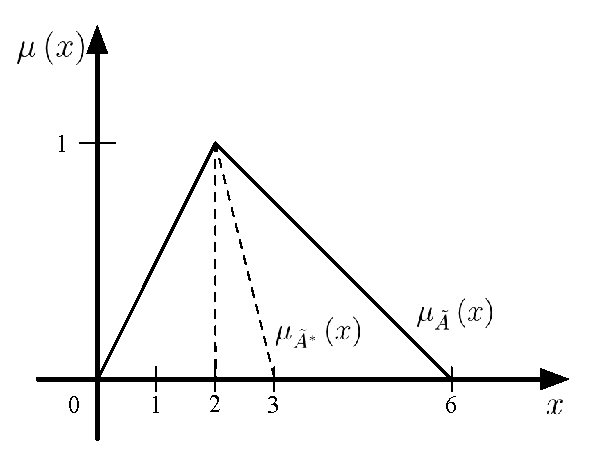
\includegraphics[width=0.85\textwidth]{sample-224}
  \end{figure}
\end{frame}

%%%%%%%%%%%%%%%%%%%%%%%%%%%%%%

\begin{frame}
  \frametitle{Представление числа}
  \begin{itemize}
    \item Не чувствительная к~знаку нечёткого числа форма  $\left\langle m_{\tilde A}, d_{\tilde A}, AS_{\tilde A} \right\rangle$; $d_{\tilde A} = a+b$; $\displaystyle AS_{\tilde A} = \frac{b-a}{2}$.
  \end{itemize}
  \begin{figure}[h]
    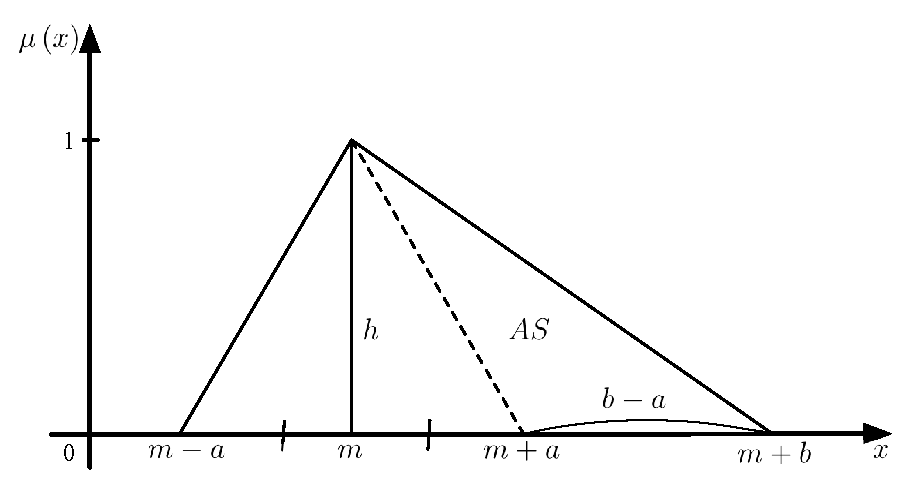
\includegraphics[width=0.9\textwidth]{as-degree}
  \end{figure}
\end{frame}

%%%%%%%%%%%%%%%%%%%%%%%%%%%%%%

\begin{frame}
  \frametitle{Свойства преобразования L}
  \begin{enumerate}
    \item Преобразование $L$ сохраняет моду нечёткого числа, т.\,е. $\forall \lambda \in \left[ 0;1 \right]:\ m_{\tilde A}=m_{\tilde A^{*}}$.
    \item При некоторых значениях параметра $\lambda$ преобразование $L$ сохраняет
      \begin{enumerate}
        \item знак степени асимметрии: $\exists \lambda \in [0;1]:\ sign(AS_{\tilde A})=sign(AS_{\tilde A^{*}})$;
        \item значение степени асимметрии: $\exists \lambda \in [0;1]:\ AS_{\tilde A}=AS_{\tilde A^{*}}$.
      \end{enumerate}
      $\displaystyle \lambda^* =\frac{a}{a+b}=\frac{a}{d_{\tilde A}}$ сохраняет значение степени асимметрии.
    \item $\forall \lambda \in \left[ 0;1 \right]: A_{\alpha}^{*}\subset A_\alpha;\ d_{\tilde A} \geqslant d_{\tilde A^{*}}$~--- преобразование~$L$ уменьшает длину носителя нечёткого числа и~оставляет $\alpha$-интервалы модифицированного числа внутри $\alpha$-интервалов исходного числа.
  \end{enumerate}
\end{frame}

%%%%%%%%%%%%%%%%%%%%%%%%%%%%%%

\begin{frame}
  \frametitle{Алгебра модифицированных нечётких чисел}
  \begin{itemize}
    \item Aлгебра $P=\left\langle K ;\ +,\,*, 0, 1 \right\rangle$, $K=\left\lbrace \bar x(\alpha) \right\rbrace$
      \begin{equation}
        \label{eq:def-one}
        \bar{x}\left( \alpha  \right)=c+k\alpha,
      \end{equation}
    \item Коэффициенты в~\eqref{eq:def-one}
      \begin{equation}
        \label{eq:modified-number-from-abm}
        \begin{aligned}
          & \left[ \begin{aligned}
          & c=m+b-\lambda \left( a+b \right) \\ 
          & k=\lambda \left( a+b \right)-b \\ 
        \end{aligned} \right. \\ 
        & \lambda \in \left[ 0;1 \right];\ c,k\in \mathbb{R} \\ 
      \end{aligned}
      \end{equation}
    \item Элементы множества $K$ линейны; достаточно знать два значения~--- $\bar{x}_{\tilde A}\left( 0 \right)$ и~$\bar{x}_{\tilde A}\left( 1 \right)=m_{\tilde A}$, чтобы найти $\tilde{A}$:
      \begin{equation}
        \label{eq:isomorphic-field}
        \bar{x}_{\tilde A}\left( \alpha \right)=\bar{x}_{\tilde A}\left( 0 \right)+\alpha \left(\bar{x}_{\tilde A}\left( 1 \right)-\bar{x}_{\tilde A}\left(0 \right) \right)=\alpha \bar{x}_{\tilde A}\left( 1 \right)+\left( 1-\alpha  \right) \bar{x}_{\tilde A}\left( 0 \right)
      \end{equation}
  \end{itemize}
\end{frame}

%%%%%%%%%%%%%%%%%%%%%%%%%%%%%%

\begin{frame}
  \frametitle{Сложение и его свойства}
  \begin{itemize}
    \item Операция сложения на~множестве $K$
      \begin{equation}
        \label{eq:fuzzy-addition}
        \bar{x}_1\left(\alpha \right)+\bar{x}_2\left(\alpha \right)=r_1\left( \alpha  \right)=c_1+c_2+\left(k_1+k_2 \right)\alpha,\ r_1 \left( \alpha  \right)\in K
      \end{equation}
    \item Нейтральный по сложению элемент
      \begin{gather}
        \label{eq:fuzzy-zero}
        \bar{0}=0+0\alpha \in K: \forall \bar{x}(\alpha )\in K: \notag \\ 
        \bar{x}(\alpha )+\bar{0}=c+k\alpha +0+0\alpha =\bar{x}(\alpha )
      \end{gather}
    \item Противоположный по сложению элемент~\eqref{eq:fuzzy-minus} 
      \begin{equation}
        \label{eq:fuzzy-minus}
        -\bar{x}\left(\alpha \right)=-c-k\alpha \in K:\ \bar{x}\left( \alpha  \right)+\left( -\bar{x}\left( \alpha  \right) \right)=\bar{0}
      \end{equation}
    \item Алгебра $\left \langle K,+,0 \right \rangle$~--- абелева группа
  \end{itemize}
\end{frame}

%%%%%%%%%%%%%%%%%%%%%%%%%%%%%%

\begin{frame}
  \frametitle{Умножение и его свойства}
  \begin{itemize}
    \item Операция умножения на~множестве $K$
      \begin{equation}
      \label{eq:fuzzy-multiplication}
        r_2\left( \alpha \right)=c_1 c_2+\left(c_1 k_2+ c_2 k_1 +k_1 k_2 \right)\alpha;\ r_2\left( \alpha  \right)\in K
      \end{equation}
    \item Нейтральный по умножению элемент
      \begin{equation}
        \label{eq:fuzzy-one}
        \bar{1}=1+0\alpha \in K:\ \forall \bar{x}\left( \alpha  \right)\in K\quad \bar{x}\left( \alpha  \right)\cdot \bar{1}=\bar{x}\left( \alpha  \right)
      \end{equation}
    \item Обратный по умножению элемент
      \begin{equation}
        \label{eq:fuzzy-division}
        \bar{x}^{-1}(\alpha )=\frac{1}{c}-\frac{k}{c\left(c+k\right)}\alpha \in K,\ c\ne 0:\ \bar{x}\left(\alpha \right){{\bar{x}}^{-1}}\left( \alpha  \right)=\bar{1}
      \end{equation}
    \item При~$c+k=m=0$~\eqref{eq:modified-number-from-abm} обратного элемента для $\bar{x}\left( \alpha  \right)$ не существует
    \item Алгебра ненулевых элементов $\left \langle K,*,1 \right \rangle$~--- абелева группа
    \item Умножение дистрибутивно относительно сложения
  \end{itemize}
\end{frame}

%%%%%%%%%%%%%%%%%%%%%%%%%%%%%%

\begin{frame}
  \frametitle{Двухточечные вычисления}
  \begin{itemize}
    \item Согласно~\eqref{eq:isomorphic-field}
      \begin{equation}
        \label{eq:isomorphic-field-shortened}
        \bar{x}_{\tilde A}\left( \alpha \right)=\alpha \bar{x}_{\tilde A}\left( 1 \right)+\left( 1-\alpha  \right) \bar{x}_{\tilde A}\left( 0 \right) \in K
      \end{equation}
    \item Для произвольной алгебраической операции~$*$
      \begin{equation}
      \label{eq:two-point-calculations}
        \bar{x}_{\tilde A}\left( \alpha \right)*\bar{x}_{\tilde B}\left(\alpha \right)=\alpha \left(\bar{x}_{\tilde A}\left( 1 \right)*\bar{x}_{\tilde B}\left(1 \right) \right)+\left(1-\alpha \right)\left(\bar{x}_{\tilde A}\left(0 \right)*\bar{x}_{\tilde B}\left(0 \right) \right)
      \end{equation}
    \item Изоморфны алгебре P
    \item Преимущества:
      \begin{itemize}
        \item решение нечёткой задачи как двух чётких при $\alpha=0$ и $\alpha=1$
        \item нет необходимости вводить отношение линейного порядка
        \item нет потребности в специализированном ПО
      \end{itemize}
  \end{itemize}
\end{frame}

%%%%%%%%%%%%%%%%%%%%%%%%%%%%%%

\begin{frame}
  \frametitle{Пример вычислений}
\end{frame}

%%%%%%%%%%%%%%%%%%%%%%%%%%%%%%

\begin{frame}
  \frametitle{Устойчивость задачи линейного программирования (ЗЛП)}
  \begin{itemize}
    \item Задача линейного программирования с нечёткими параметрами
    \begin{equation}
      \label{eq:fuzzy-lp-unstable-problem}
      \left\{ \begin{aligned}
        & f\left( \mathbf{x} \right)=\mathbf{Cx}\to \min;  \\ 
        & \mathbf{Ax}=\mathbf{B},
      \end{aligned} \right.
      \to
      \left\{ \begin{aligned}
        & f\left( \mathbf{x} \right)={\mathbf{C}^{*}}\mathbf{x}\to \min;  \\ 
        & {\mathbf{A}^{*}}\mathbf{x}={\mathbf{B}}^{*},
      \end{aligned} \right.
    \end{equation}
    $\mathbf{A}^{*}=\left\{ \bar{x}_{\tilde{A}_{ij}}\left(\alpha \right) \right\}$, $\mathbf{B}^{*}=\left\{ \bar{x}_{\tilde{B}_i}\left(\alpha \right) \right\}$, $\mathbf{C}^{*}=\left\{ \bar{x}_{\tilde{C}_i}\left(\alpha \right) \right\}$
    \item Невозмущённое решение~--- при $\alpha=1$ (свойство сохранения моды)
    \item Задача устойчива, если результат получается в той же форме, что и исходные данные (не происходит искажений формы нечётких чисел)
    %    \item Предлагаемое условие устойчивости по решению:
%      \begin{equation}
%      \label{eq:fuzzy-solution-stability}
%        \forall \varepsilon >0\, \exists \delta >0:\forall \alpha \in \left[0; 1\right)\,\left| \alpha -1 \right|<\delta \linebreak \Rightarrow \left\| \mathbf{x}\left( 1 \right)-\mathbf{x}\left( \alpha  \right) \right\|<\varepsilon
%      \end{equation}
  \end{itemize}
\end{frame}

%%%%%%%%%%%%%%%%%%%%%%%%%%%%%%

\begin{frame}
  \frametitle{Устойчивость ЗЛП}
  \begin{itemize}
    \item При $\alpha=0$, все~значения $\lambda_S$ ($S$~--- индекс $\tilde A_{ij}$, $\tilde B_i$, $\tilde C_i$)~--- принимают граничные значения (0 или 1). 
    \item Ограничения на $\lambda$ для минимизации потерь экспертной информации
      \begin{equation}
      \label{eq:lambda-minimization-criterion}
        {\left( \lambda_{S}^{\star}-\lambda_S \right)}^2\to \min
      \end{equation}
    \item Задача векторной оптимизации ввиду противоречивости критерия~\eqref{eq:lambda-minimization-criterion} и~целевой~функции задачи~\eqref{eq:fuzzy-lp-unstable-problem}
    \item Применяется аддитивная свёртка критериев в~целевой функции~\eqref{eq:modified-target-function}
      \begin{equation}
      \label{eq:modified-target-function}
        f^{*}\left( \mathbf{x} \right)=\mathbf{C}^{*}\mathbf{x}+\gamma \sum\limits_{s}^{}{\left(\lambda_{S}^{*}-\lambda_S \right)}^{2} \to \min
      \end{equation}
  \end{itemize}
\end{frame}

\begin{frame}
  \frametitle{Задача сетевого планирования}
  \begin{figure}
    \center
    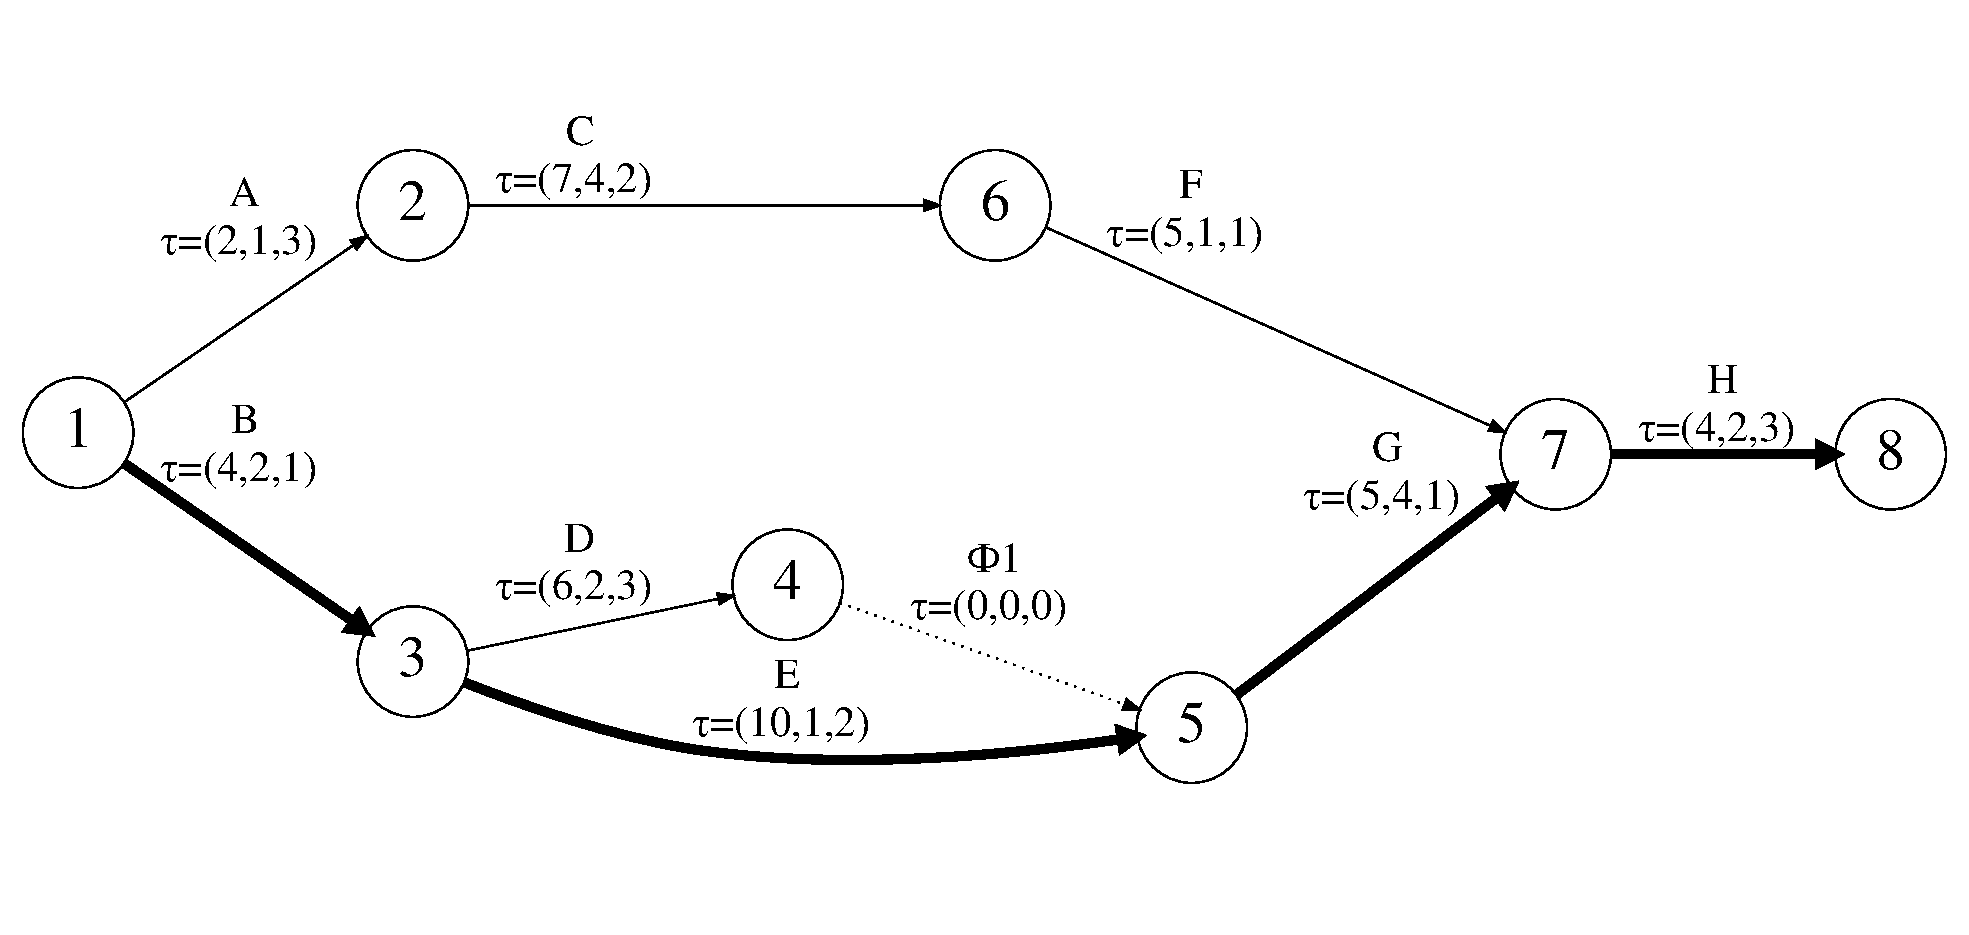
\includegraphics[width=\textwidth]{pplan}
  \end{figure}
  $G=(V,E)$, $\left| V \right|=n$, $\left| E \right|=m$; \\
  дуги $e_j$~--- работы $w_j$, длительностью $\tau_j$, $j=\overline{1,m}$; \\
  вершины $v_i$~--- события $z_i$ с~временами наступления $t_i$, $i=\overline{1,n}$
\end{frame}

%%%%%%%%%%%%%%%%%%%%%%%%%%%%%%

\begin{frame}
  \frametitle{Модифицированная задача сетевого планирования}
  \begin{itemize}
    \item ЗЛП с~нечёткими временными оценками
      \begin{equation}
      \label{eq:modified-fcpm-lp}
        \left\{ \begin{aligned}
          & T(\alpha )=t_n-t_1\to \min  \\ 
          & t_{j_s}-t_{i_s}\geqslant \bar{\tau}_s\left(\alpha,\lambda_s \right),\ \forall s=\overline{1,m}.
        \end{aligned} \right.
      \end{equation}
    \item При $\alpha = 0$ решается возмущённая задача
      \begin{equation}
      \label{eq:modified-fcpm-lp-alpha}
        \left \{ \begin{aligned}
          & T^* \left(\alpha, \lambda \right) = t_n-t_1+\gamma \sum \limits_{s=1}^{m} \left(\lambda_s^*-\lambda_s \right)^2 \to \min; \\
          & t_{j_{s_1}}-t_{i_{s_1}} = \bar{\tau}_{s_1}\left(\alpha, \lambda_{s_1} \right),\ \forall s_1 \in S_1\left(1\right); \\
          & t_{j_s}-t_{i_s} \geqslant \bar{\tau}_s\left(\alpha, \lambda_s \right),\ \forall s \notin S_1\left(1\right),\,s=\overline{1,m}.
        \end{aligned} \right.
      \end{equation}
    \item Результат~--- совокупность $\left \langle \tilde T, S_1, \lambda \right \rangle$
  \end{itemize}
\end{frame}

%%%%%%%%%%%%%%%%%%%%%%%%%%%%%%

\begin{frame}
  \frametitle{Решение примера (с. 19)}
  \begin{itemize}
    \item При~$\alpha=1$: $T\left( 1 \right)=23$, $S_1\left( 1 \right)=\left\{ B,E,G,H \right\}$
    \item При~$\alpha=0$ и $\gamma \sim 10$: $T^*\left( 0 \right)=20,83$, $S_1\left( 0 \right)=\left\{ B,E,G,H \right\}$
      \begin{equation}
      \label{eq:0-level-fcpm-task}
        T\left( 0 \right)=t_8-t_1+\gamma \sum\limits_{s=A}^{H}\left( \lambda_{s}^{*}-\lambda_s \right)^{2}\to \min
      \end{equation}
      \begin{equation}
      \label{eq:0-level-fcpm-constraints}
        \left\{ \begin{aligned}
          & t_2-t_1 \geqslant 5-4\lambda_A \\ 
          & t_6-t_2 \geqslant 9-6\lambda_C \\ 
          & t_4-t_3 \geqslant 9-5\lambda_D \\ 
          & t_5-t_4 \geqslant 0 \\ 
          & t_7-t_6 \geqslant 6-2\lambda_F \\ 
        \end{aligned} \right.
        \left\{ \begin{aligned}
          & t_3-t_1=5-3\lambda_B \\ 
          & t_5-t_3=12-3\lambda_E \\ 
          & t_7-t_5=6-5\lambda_G \\ 
          & t_8-t_7=7-5\lambda_H
        \end{aligned} \right.
      \end{equation}
    \item Окончательный результат: $S_1=\left\{ B,E,G,H \right\}$, $T\left( \alpha \right)=20,67+2,33\alpha$, $\lambda =\left\{ 0,25;\ 0,68;\ 0,67;\ 0,4;\ 0,35;\ 0,5;\ 0,83;\ 0;43 \right\}$
  \end{itemize}
\end{frame}

\begin{frame}
  \frametitle{Программное обеспечение}
  Приложение <<CSBusinessGraph>> выполняет все вычисления только с использованием действительных переменных
  \begin{figure}
    \center
    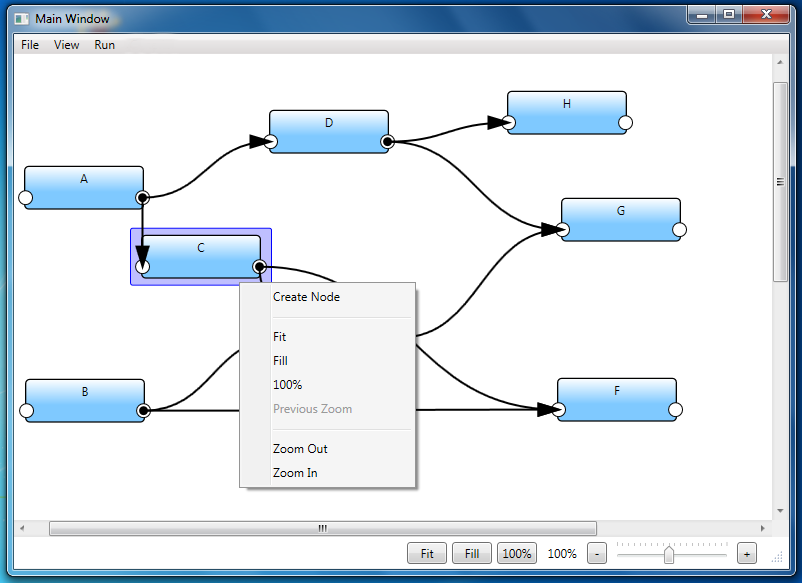
\includegraphics[width=0.8\textwidth]{app-sample-graph.png}
  \end{figure}
\end{frame}

%%%%%%%%%%%%%%%%%%%%%%%%%%%%%%

\begin{frame}
  \frametitle{Результаты работы}
  \begin{itemize}
    \item Комплекс методов для моделей с чёткими отношениями и нечёткими параметрами
    \begin{itemize}
      \item применение классических методы решения
      \item достижение требуемых качественных свойств решения
    \end{itemize}
    \item Параметрическая модель представления нечёткого числа
    \begin{itemize}
      \item максимальное сохранение экспертной информации
      \item двухточечные вычисления~--- эффективная численная реализации решения
    \end{itemize}
    \item Устойчивость решения задачи линейного программирования с нечёткими параметрами
    \begin{itemize}
      \item свёртка критериев для управления устойчивостью
      \item алгоритм получения устойчивого решения задачи
    \end{itemize}
    \item Апробация методов~--- задача сетевого планирования
    \item Программный комплекс~--- решение задачи оценки сроков разработки программного обеспечения
  \end{itemize}
\end{frame}

%%%%%%%%%%%%%%%%%%%%%%%%%%%%%%

\begin{frame}
  \frametitle{Апробация работы и публикации}
  Основные положения работы докладывались на конференциях:
  \begin{itemize}
    \item Современные проблемы прикладной математики, теории управления и математического моделирования (Воронеж, 2012 г.)
    \item Информатика: проблемы, методология, технологии (Воронеж, 2013--2014 гг.);
    \item Современные технологии в задачах управления, автоматики и обработки информации (Алушта, 2013--2014 гг.);
    \item Радиоэлектроника, электротехника и энергетика (Москва, 2014).
  \end{itemize}
  Основное содержание диссертационного исследования изложено в 11 научных работах, из~них 4 статьи в~изданиях, рекомендованных ВАК РФ.
\end{frame}

\end{document} 